\documentclass[zihao=false,fontset=windows]{ctexart}
% ctexart 不接受任意 pt 选项。正文改 {10pt}，方括号里是行距。
\usepackage{scrextend}
\changefontsizes[12pt]{10pt}

\usepackage[a4paper,left=2.35cm,right=2.35cm,top=1.7cm,bottom=1.9cm]{geometry}
\usepackage{xcolor}
\usepackage{graphicx}
\usepackage{amsmath,amssymb}
\usepackage{enumitem}
\usepackage{tabularx}
\usepackage{colortbl}
\usepackage{listings}
\usepackage{hyperref}
\usepackage[most]{tcolorbox}

\definecolor{feishuText}{RGB}{31,35,41}
\definecolor{feishuBlue}{RGB}{36,91,219}
\definecolor{feishuRed}{RGB}{216,57,49}
\definecolor{feishuGray}{RGB}{100,106,115}
\definecolor{feishuGray2}{RGB}{143,149,158}
\definecolor{feishuPinkBg}{RGB}{251,191,188}
\definecolor{quoteBar}{RGB}{51,112,255}
\definecolor{codebg}{RGB}{245,246,247}
\definecolor{codeborder}{RGB}{222,224,227}
\definecolor{inlinebg}{RGB}{242,243,245}
\definecolor{callRed}{RGB}{253,226,226}
\definecolor{callOrange}{RGB}{255,245,235}
\definecolor{callYellow}{RGB}{254,255,240}
\definecolor{callGreen}{RGB}{240,251,239}
\definecolor{callBlue}{RGB}{240,244,255}
\definecolor{callRedSoft}{RGB}{254,241,241}
\definecolor{callSun}{RGB}{255,255,204}
\definecolor{tableHead}{RGB}{242,243,245}
\definecolor{tableRule}{RGB}{222,224,227}
\definecolor{codeText}{RGB}{31,35,41}
\definecolor{codeKeyword}{RGB}{0,0,255}
\definecolor{codeComment}{RGB}{0,128,0}
\definecolor{codeString}{RGB}{163,21,21}

\setmainfont{Times New Roman}
\setCJKmainfont{Microsoft YaHei}[AutoFakeBold=2.2]
\setCJKsansfont{Microsoft YaHei}[AutoFakeBold=2.2]
\setCJKmonofont{Microsoft YaHei}[AutoFakeBold=2.2]
\setmonofont{Consolas}
\newfontfamily\emojifont{Segoe UI Emoji}

\hypersetup{
  colorlinks=true,
  urlcolor=feishuBlue,
  linkcolor=feishuBlue,
  unicode=true,
  pdftitle={SoViT}
}

\setlength{\parindent}{0pt}
\setlength{\parskip}{0.42em}
\setlength{\fboxsep}{1.5pt}
\setlength{\emergencystretch}{3em}
\linespread{1.28}
\color{feishuText}
\arrayrulecolor{tableRule}
\urlstyle{same}

\setlist[enumerate]{label=\textcolor{feishuBlue}{\arabic*.}, leftmargin=1.7em, itemsep=0.22em, topsep=0.28em, parsep=0.08em, partopsep=0pt}
\setlist[itemize,1]{label=\textcolor{feishuBlue}{\textbullet}, leftmargin=1.35em, itemsep=0.18em, topsep=0.25em, parsep=0.06em, partopsep=0pt}
\setlist[itemize,2]{label=\textcolor{feishuBlue}{◦}, leftmargin=1.45em, itemsep=0.12em, topsep=0.15em}
\setlist[itemize,3]{label=\textcolor{feishuBlue}{\rule[0.18em]{0.38em}{0.38em}}, leftmargin=1.55em, itemsep=0.1em, topsep=0.12em}

\newcommand{\feiEmoji}[1]{{\emojifont #1}}
\newcommand{\incode}[1]{\colorbox{inlinebg}{\ttfamily\small #1}}
\newcommand{\bigmath}[1]{%
  \begin{center}\large$\displaystyle #1$\end{center}%
}

\lstset{
  language=Python,
  basicstyle=\ttfamily\footnotesize\color{codeText},
  keywordstyle=\color{codeKeyword},
  commentstyle=\color{codeComment},
  stringstyle=\color{codeString},
  showstringspaces=false,
  breaklines=true,
  columns=fullflexible,
  keepspaces=true,
  tabsize=4,
  upquote=true,
  aboveskip=2pt,
  belowskip=0pt,
  xleftmargin=0pt,
  frame=none
}

\tcbset{
  feishubase/.style 2 args={
    enhanced,
    boxrule=0pt,
    arc=8pt,
    left=10pt,
    right=10pt,
    top=7pt,
    bottom=7pt,
    before skip=6pt,
    after skip=6pt,
    colback=#1,
    colframe=#1,
    before upper={\feiEmoji{#2}\hspace{0.45em}\ignorespaces}
  }
}
\newtcolorbox{feishubox}[2]{feishubase={#1}{#2}, breakable}
\newtcolorbox{feishuboxnb}[2]{feishubase={#1}{#2}}

\newtcolorbox{feishuquote}{
  enhanced,
  breakable,
  boxrule=0pt,
  leftrule=3pt,
  arc=0pt,
  colframe=quoteBar,
  colback=white,
  left=8pt,
  right=2pt,
  top=2pt,
  bottom=2pt,
  before skip=4pt,
  after skip=4pt,
  before upper=\color{feishuGray}
}

\newtcolorbox{feishucode}{
  enhanced,
  breakable,
  colback=codebg,
  colframe=codeborder,
  boxrule=0.6pt,
  arc=6pt,
  left=6pt,
  right=6pt,
  top=5pt,
  bottom=4pt,
  before skip=6pt,
  after skip=6pt
}

\usepackage{needspace}

% 来源：https://scnajei2ds6y.feishu.cn/wiki/FPZRwVpY1iNH39k67RscHYuOn5e

% 公式按网页渲染人工转写并视觉核对；图2/3采用已实际查看的正常网页截图裁取。

\begin{document}

{\zihao{1}\bfseries SoViT\par}


\begin{feishubox}{callOrange}{📚}
论文：《Getting ViT in Shape: Scaling Laws for Compute-Optimal Model Design》\par 论文链接：\href{https://arxiv.org/pdf/2305.13035}{https://arxiv.org/pdf/2305.13035}
\end{feishubox}

\par\needspace{5\baselineskip}\vspace{1em}\noindent{\zihao{-2}\bfseries \textcolor{feishuBlue}{1.} 背景}\par\vspace{0.28em}

在此前对LLM的研究中，Scaling Law能够给出在给定的计算下，最佳模型的参数量。SoViT在此基础上做了两件事：\par

\begin{itemize}

\item 将Scaling Law的视角引入到ViT上。

\item 考虑内部维度形状（即Width、Depth和 MLP dim）随计算量（GFLOPs）关系。

\end{itemize}

\begin{center}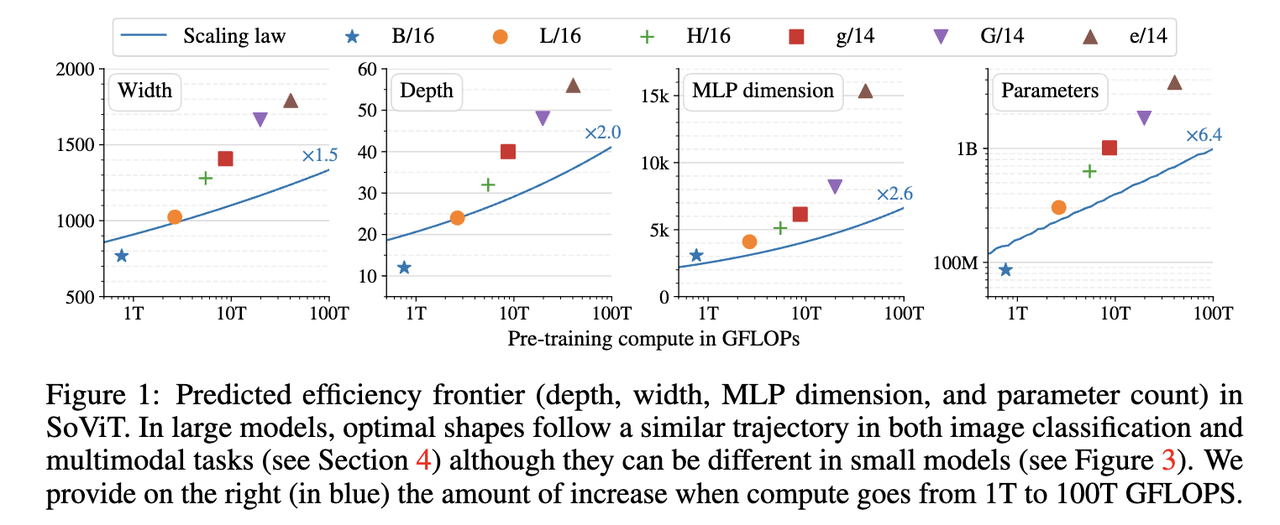
\includegraphics[width=0.98\linewidth]{images/SoViT/fig-01.png}\end{center}

从上图可以看到：\par

\begin{itemize}

\item 当计算量（GFLOPs）提高时，最优的模型对于Width、Depth和 MLP dim有不同的缩放比率。

\item 现在主流的ViT架构都是参数量冗余的（Shape不是最优）

\end{itemize}

\par\needspace{5\baselineskip}\vspace{1em}\noindent{\zihao{-2}\bfseries \textcolor{feishuBlue}{2.} Scaling Strategy}\par\vspace{0.28em}

\par\needspace{5\baselineskip}\vspace{1em}\noindent{\zihao{3}\bfseries \textcolor{feishuBlue}{2.1} 问题描述}\par\vspace{0.28em}

我们首先对问题作一个形式化描述。我们用一个元组$x=(x_1,x_2,\ldots,x_D)\in\mathbb N^D$来表示一个神经网络的“形状”（即若干维度），例如宽度（width）、深度（depth）、MLP 的隐藏维度（MLP dim）等。我们用 t 表示训练计算量（例如 GFLOPs）。我们令 $f:\mathbb N^D\times\mathbb R_+\to\mathbb R$ 表示一个关心的性能度量（performance metric），如下游任务的误差率（例如 ImageNet 10-shot 误差）。具体地，$f(x,t)$ 指：在一个给定的计算预算 $t$ 下训练形状为 $x$ 的网络，并测量得到的性能（通常是一个Loss，值越低越好）。\par

\textcolor{feishuRed}{\textbf{我们的目标是：给定一个固定的计算预算 }}{\boldmath$t$}\textcolor{feishuRed}{\textbf{，找到一个最优的形状 }}{\boldmath$x^\star$}\textcolor{feishuRed}{\textbf{（该 }}{\boldmath$x^\star$}\textcolor{feishuRed}{\textbf{ 将随 }}{\boldmath$t$}\textcolor{feishuRed}{\textbf{ 的变化而变化），使得：}}\par

{\boldmath\bigmath{f(x^\star,t)-\inf_{x\in\mathbb N^D}f(x,t)\leq\epsilon\textcolor{feishuRed}{,}}}

\textcolor{feishuRed}{\textbf{其中 }}{\boldmath$\epsilon$}\textcolor{feishuRed}{\textbf{ 是一个很小的容忍度。由于实验测量、建模近似以及可试验的模型是有限的，我们无法期待 }}{\boldmath$\epsilon=0$}\textcolor{feishuRed}{\textbf{，因此需要允许一定的性能损失 }}{\boldmath$\epsilon$}\textcolor{feishuRed}{\textbf{。}}\par

\par\needspace{5\baselineskip}\vspace{1em}\noindent{\zihao{3}\bfseries \textcolor{feishuBlue}{2.2} 单一形状维度的情况}\par\vspace{0.28em}

在视觉 Transformer 中，仅仅改变网络的形状（例如宽度、深度、MLP 大小）就会显著影响它预训练后的下游表现。为了确定形状如何随计算量一起按比例扩展（scale up），让我们先考虑只有一个形状维度 $x_k$。类似于先前的一些工作，当考虑到计算量 $t$ 时，人们往往需要跑大量实验来在不同 $x_k$ 上找出优的 Pareto optimal frontier，并从中拟合出幂律关系，\textbf{然而这种做法代价昂贵。}\par

为此，SoViT提出以下联合函数形式，用来同时考虑模型尺寸和训练计算量：\par

\bigmath{f_k(x_k,t)\sim\alpha_kx_k^{-a_k}+(\beta_kx_k^{b_k}+\xi_k)t^{-c}+\varepsilon_k,}

其中 $\alpha_k,a_k,\beta_k,b_k,c,\xi_k,\varepsilon_k>0$。$a_k$ 表示在“无计算限制”的情形下，当改变对应形状维度时所出现的“幂律指数”；$c$ 则是表示数据规模幂律的指数；而 $b_k$ 则反映了该形状维度对整体计算量（compute）所造成的影响。上式中，$f_k$ 只聚焦维度 $k$，假设其他维度不会成为瓶颈（即它们足够大），并且假设数据量是充足的（不会过拟合）。\textcolor{feishuRed}{\textbf{随后我们会借助实验数据来拟合其中的参数。}}\par

直观而言，这个形式可从以下几点来理解：\par

\begin{enumerate}

\item \textbf{计算量无上限时}：假设训练可以无限长，则可得到熟悉的模型尺寸幂律关系

$f_k(x_k)\sim\alpha_kx_k^{-a_k}+\varepsilon_k$。这里的 $\varepsilon_k$ 表示无法再降低的那部分损失。但是无限增大$x_k$无法使得$f_k(x_k)\sim\varepsilon_k$因为联合函数的第二项会暴增。\par

\item \textbf{固定模型尺寸时}：公式只随 $t$（可视为相当于数据大小）变化，就会呈现 $\sim At^{-c}+B$ 的幂律关系；这与许多先前关于数据规模定律（data scaling laws）的观察一致。

\item \textbf{对固定计算量}$t$\textbf{而言}，$f_k(x_k,t)$ 关于 $x_k$ 的曲线并非简单的单调，而是先下降后上升，呈现准凸（quasiconvex）形状（参考右侧 IsoFlop 曲线）。这意味着若把所有其他量都固定，盲目加大某个维度到某点后，实际可能会伤害最终性能。

\item \textbf{不互相矛盾}：若把这种分维度的函数形式通用化到多个维度，理论上也不会相互冲突，因为其可以写成一个可分解的加和式（见\href{https://arxiv.org/pdf/2305.13035}{论文}附录），且根据对数据流形维度的空间划分推断，$c$这个指数在所有维度上都是一致的。

\item \textbf{在可用计算固定时的最优}$x_k$：我们可以解析出最优值

\bigmath{x_k^\star=\left(\frac{\alpha_ka_kt^c}{\beta_kb_k}\right)^{\frac{1}{b_k+a_k}}=O(t^{s_k}),}

其中$s_k=\frac{c}{b_k+a_k}.$\par

这告诉我们：在计算预算 $t$ 按某个比例增大时，最优的某个维度 $x_k$ 大致按 $t^{s_k}$ 的幂律方式增长。因为 $a_k,b_k,c>0$，所以 $s_k$ 为正。\par

\item \textbf{在最优曲线（或最优前沿）上}，可将上式带回到 $f_k$ 中，得到

\bigmath{f_k(x_k,t)=Fx_k^{-a_k}+Gt^{-c}+\varepsilon_k,}

这与之前在语言模型中观察到的“在最优前沿时，损失是模型大小和计算量各自幂律之和”的结论一致。\par

\end{enumerate}

\par\needspace{5\baselineskip}\vspace{1em}\noindent{\zihao{3}\bfseries \textcolor{feishuBlue}{2.3} 多维度情况}\par\vspace{0.28em}

SoViT 把这一思路推广到多个形状维度（如同时包含深度、宽度、MLP 大小等）。SoViT 用更少的实验就能定位到大致的最优形状。\par

\par\needspace{5\baselineskip}\vspace{1em}\noindent{\zihao{4}\bfseries \textcolor{feishuBlue}{2.3.1} Star Sweep（星形搜索）}\par\vspace{0.28em}

如果我们想在 $D$ 个不同的形状维度上做全面网格搜索，那么需要 $O(2^D)$ 个实验，这在实践中非常昂贵。为此，我们的做法是仅做“星形搜索”——即选定一个“中心”形状 $x^{(c)}$（各维都相对较大），随后“只动一个维度、保持其他不变”，并在这个维度上取一个按指数刻度排列的网格点来训练与测量，从而拟合式中的参数（特别是上文提到的 $s_k$）。例如在我们实验中，要拟合宽度 $s_{\mathrm{width}}$ 时，就把深度和 MLP 大小都固定在较大的中心值，分别训练宽度从小到较大的几种取值；对深度、MLP 也依此类推。\par

\par\needspace{5\baselineskip}\vspace{1em}\noindent{\zihao{4}\bfseries \textcolor{feishuBlue}{2.3.2} Grid Sweep（小模型网格搜索）}\par\vspace{0.28em}

在上一步我们主要是估算每个维度各自的幂指数 $s_k$，而大模型中心点 $x^{(c)}$ 仅仅是为了确保它不会形成瓶颈。然而，当我们最终要获得一个“从小到大都最优”的完整形状扩展策略时，还需要知道在“小计算量”下的最优形状是什么。如果这个初始形状选得不佳，会在往后累加时造成偏离。\par

因此我们的第二步是：专门针对小模型、短训练（即计算量不大的情形）做一个更细致的网格搜索，从而找出在这部分计算量区间的 Pareto 最优形状 $x^{(0)}$。这样一来，这个小模型的“最优形状”就能作为后续向大规模延伸的起点，我们也就同时拿到式中可能涉及的系数，保证继续往大模型方向扩展时不会过早失真。\par

\par\needspace{5\baselineskip}\vspace{1em}\noindent{\zihao{4}\bfseries \textcolor{feishuBlue}{2.3.3} 形状扩展策略}\par\vspace{0.28em}

有了上面两个要点后，我们的总体做法如下：\par

\begin{itemize}

\item 首先，用“小模型网格搜索”来获得一个在计算量 $t^{(0)}$ 下的最优形状 $x^{(0)}$。

\item 如果我们将计算量增加一个因子 $\tau$（即由 $t^{(0)}$ 变为 $\tau\cdot t^{(0)}$），则根据前面结论，每个维度可大体按 $x_k\propto t^{s_k}$ 来扩张。

\item 为简化，我们可以令所有维度在对数坐标上平均增长：比如说把 $\tau$ 分解为若干子增量，使各维度的乘法扩展在对数空间里相加即得 $\tau$，从而每次的伸缩是固定倍数。但仍可考虑更灵活的做法，分配不同的增量权重 $\omega_k$，如果有需求想要更快地扩张深度或是 MLP 等。

\end{itemize}

在SoViT的实验中采用了最简单且行之有效的方法，即让所有维度按照相同的对数步长增长。\par

\par\needspace{5\baselineskip}\vspace{1em}\noindent{\zihao{-2}\bfseries \textcolor{feishuBlue}{3.} 实验}\par\vspace{0.28em}

\par\needspace{5\baselineskip}\vspace{1em}\noindent{\zihao{3}\bfseries \textcolor{feishuBlue}{3.1} Image Classification}\par\vspace{0.28em}

ViT-g/14参数量1B、ViT-L/16参数量300M。相比之下SoViT-400m/14效果最佳。\par

\begin{center}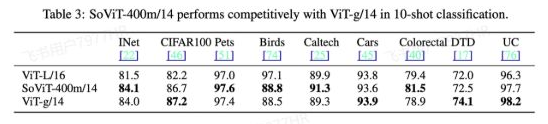
\includegraphics[width=0.78\linewidth]{images/SoViT/fig-02.png}\end{center}

\par\needspace{5\baselineskip}\vspace{1em}\noindent{\zihao{3}\bfseries \textcolor{feishuBlue}{3.2} Multitask Decoding}\par\vspace{0.28em}

这些任务就是接上Decoder之后进行测评的，也最能表现SoViT在现在的vlm中的优越性：\par

\begin{center}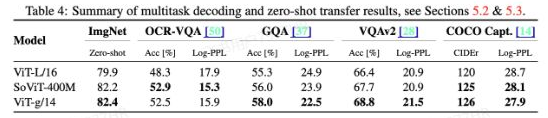
\includegraphics[width=0.78\linewidth]{images/SoViT/fig-03.png}\end{center}

\end{document}
